\documentclass{article}
\usepackage{graphicx}  % Per le immagini
\usepackage{float}      % Per il posizionamento delle figure

\title{Grafici}
\author{GIUSEPPE CALABRESE}
\date{February 2025}

\begin{document}

\begin{figure}[H]
    \centering
    
\includegraphics[width=0.5\linewidth]{Logo Unicam/unicam.jpg}
    \label{fig:logo}
\end{figure}

\centering
{\Large \textbf{Università degli Studi di Camerino}     \par
    \vspace{1 cm}
        \Large \textbf{Scuola di Scienze e Tecnologie}  \par
        \Large \textbf{Algoritmi e Strutture Dati}      \par
    \vspace{3 cm}
        \Large \textbf{GRAFICI SULLA VALUTAZIONE NUMERICA DELLE PRESTAZIONI} \par
    \vspace{1 cm}
        \Large \textbf{Giuseppe Calabrese (Matricola 122630)}
}

\newpage

% Primo set di grafici
\section*{Numero di confronti}
\begin{figure}[H]
    \centering
    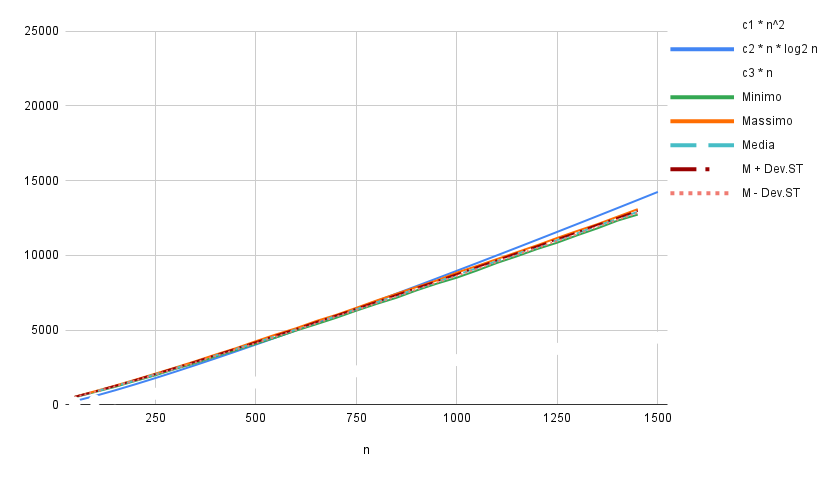
\includegraphics[width=0.98\linewidth]{Grafici/AVLTreeSort.png}
    \caption{Numero di confronti per AVLTreeSort}
    \label{fig:avl_confronti}
\end{figure}

\begin{figure}[H]
    \centering
    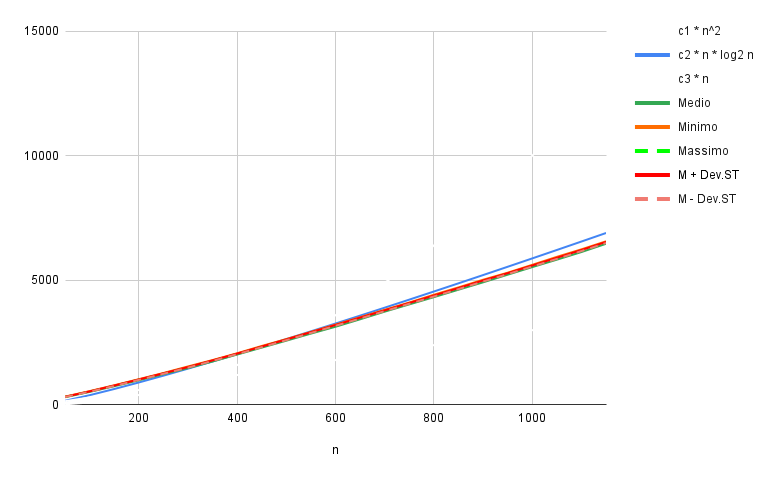
\includegraphics[width=0.98\linewidth]{Grafici/Heap3SortConf.png}
    \caption{Numero di confronti per Heap3Sort}
    \label{fig:heap_confronti}
\end{figure}

\newpage

% Secondo set di grafici
\section*{Tempi di esecuzione}
\begin{figure}[H]
    \centering
    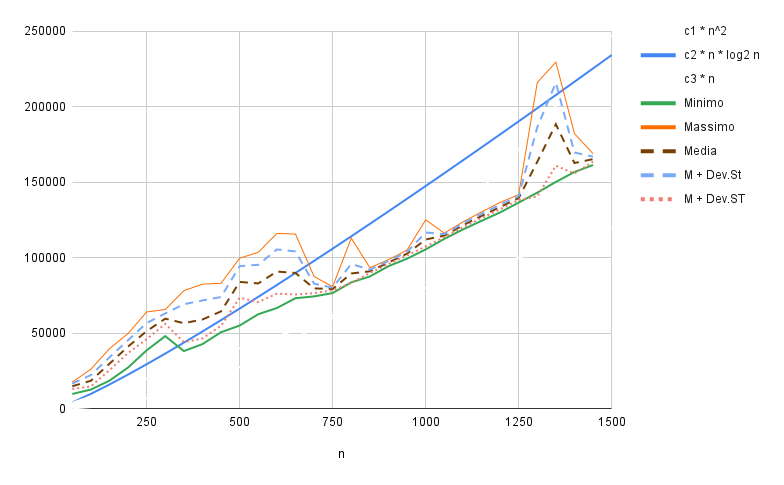
\includegraphics[width=0.95\linewidth]{Grafici/Heap3SortTempNs.png}
    \caption{Heap3Sort tempo di esecuzione in nanosecondi}
    \label{fig:heap_tempo}
\end{figure}

\begin{figure}[H]
    \centering
    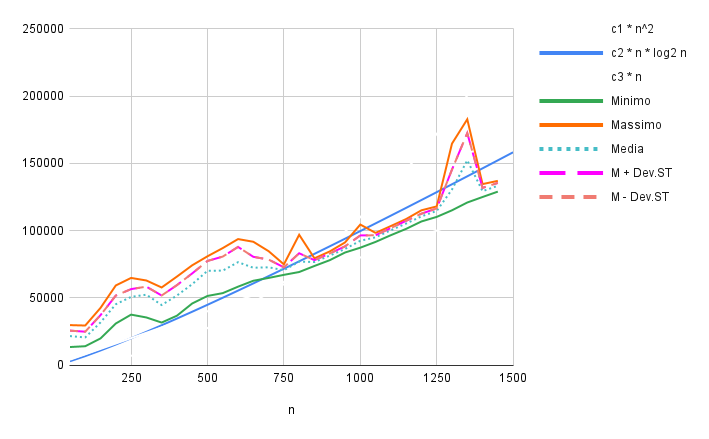
\includegraphics[width=0.95\linewidth]{Grafici/AVLTreeSortTempNs.png}
    \caption{AVLTreeSort tempo di esecuzione in nanosecondi}
    \label{fig:avl_tempo}
\end{figure}

\newpage

% Terzo set di grafici
\section*{Confronto tra AVL e Heap}
\begin{figure}[H]
    \centering
    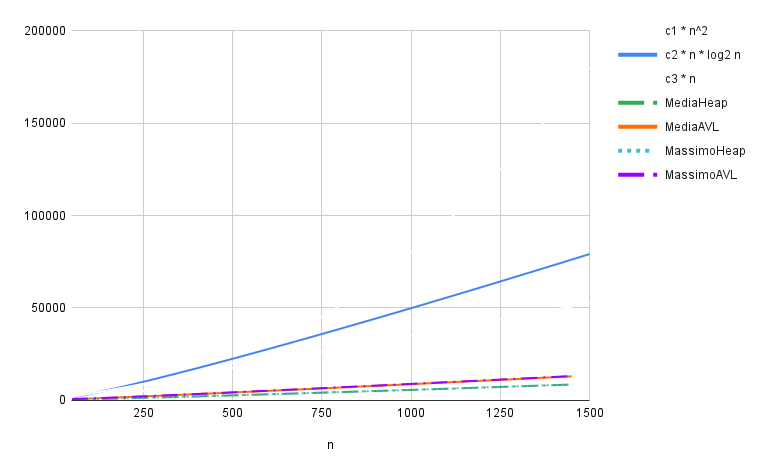
\includegraphics[width=0.95\linewidth]{Grafici/AVLvsHEApNc.png}
    \caption{Confronto AVL vs Heap: caso medio e massimo per numero di confronti}
    \label{fig:confronto_nc}
\end{figure}

\begin{figure}[H]
    \centering
    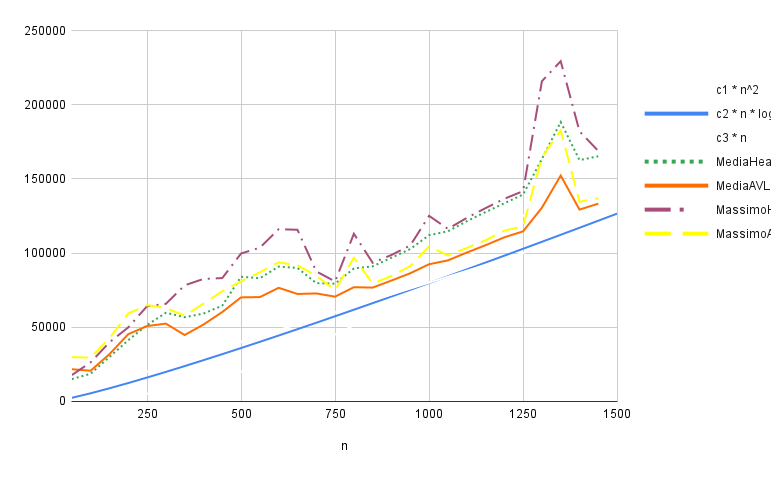
\includegraphics[width=0.95\linewidth]{Grafici/AVLvsHeapTs.png}
    \caption{Confronto AVL vs Heap: caso medio e massimo per tempo di esecuzione}
    \label{fig:confronto_ts}
\end{figure}

\end{document}
